%%%%%%%%%%%%%%%%%%%%%%%%%%%%%%%%%%%%%%%%%%%%%%%%%%%%%%%%%%%%%%%%%%%%%%%%%%%
%   导言区
\documentclass[12pt, a4paper]{ctexart}
\usepackage{amsmath, amsthm, amssymb, appendix, cite, xcolor, multirow, multicol, makecell}
\usepackage{bm, graphicx, mathrsfs, geometry, listings, framed, booktabs, qtree, tikz, tikz-qtree}
\usepackage[CJKbookmarks=true]{hyperref}

\AtBeginDocument {
\addtolength{\abovedisplayskip}{-2ex}
\addtolength{\abovedisplayshortskip}{-2ex}
\addtolength{\belowdisplayskip}{-2ex}
\addtolength{\belowdisplayshortskip}{-2ex}
}

\newcommand{\upcite}[1]{\textsuperscript{\cite{#1}}}
\newcommand{\upref}[1]{\textsuperscript{\ref{#1}}}

\title{\LaTeX\textbf{学习报告}}
\author{Shiyuu}
\date{\today}
%\advisor{}

\linespread{0.5}    %设置{n}倍行距
\geometry{left=1.0cm, right=1.0cm, top=0.5cm, bottom=0.5cm}%设定页边距
%\advisor{}

\linespread{1.45}    %设置{n}倍行距
\geometry{left=2cm, right=2cm, top=2cm, bottom=2cm}%设定页边距

%lst代码设定(tex)
\lstset
{%   
    language=tex,
    basicstyle=\tt,
    showstringspaces=false,
    numbers=left,
    stepnumber=1, 
    numbersep=2pt,
    xleftmargin=1em,
}

%%%%%%%%%%%%%%%%%%%%%%%%%%%%%%%%%%%%%%%%%%%%%%%%%%%%%%%%%%%%%%%%%%%%%%%%%%%
\begin{document}
\maketitle
\setcounter{page}{-1}
\maketitle
\thispagestyle{empty}
\begin{center}
    \rule[-10pt]{16cm}{0.05em}
\end{center}%一条不错的加横线指令
\begin{abstract}
这一篇文档算不上是什么报告,其实只是拿浅薄的积累来练个手(毕生所学),以及把平常用的{\TeX}方法列个表出来方便查阅。最重要的还是把从{\href{https://www.zhihu.com/people/dylan-dong-233}{数院学长}}那里薅来的我根本搞不懂的{\TeX}模板做个参考,免得以后Compile了一大堆错误都不知道为什么。

现阶段没有太多时间去学{\TeX}的高端用法真是抱歉,反正能记笔记、交作业就行,后面有时间再补充。如果不耐烦了可以直接跳到{\nameref{sec:preset}}介绍部分喵。
\end{abstract}

\begin{center}
    \rule[-10pt]{16cm}{0.05em}
\end{center}%一条不错的加横线指令

%\newpage
\tableofcontents
\newpage
%开个目录

%%%%%%%%%%%%%%%%%%%%%%%%%%%%%%%%%%%%%%%%%%%%%%%%%%%%%%%%%%%%%%%%%%%%%%%%%%%
\section{文本}
那既然{\LaTeX}是用来写字的,那么文本编辑好像也没什么好说的,直接往{\textbackslash}article{}里面敲字就行了。一篇最普通的文章模板(例如artical、ctexart)理论上就只需要
\begin{framed}
\begin{lstlisting}[language=tex]
    \begin{doucument}
        .......
    \end{document}
\end{lstlisting}
\end{framed}
这一段环境就可以了,在省略号省略的部分,直接往里敲文字就可以。

当然,只有文章题目是不够的的,我们还需要更多的一级、二级、三级标题。只需要下面这几个命令(不用end)

\begin{framed}
\begin{lstlisting}[language=tex]
        \section{Sec:A}
            \subsection{Sec:A-1}
                \subsubsection{Sec:A-1.1}
                \sunsubsection*{notitle}
\end{lstlisting}
\end{framed}

以此类推,{\TeX}会自动帮你编号,{\{\}}中的就是章节名称,一般情况下三级标题也够用了,如果还要加的话可以在里面内嵌{\textbackslash}box、{\textbackslash}framed之类的环境,然后使用{\textbackslash}label和{\textbackslash}ref交叉引用。

前面还有模板之类的问题,其实对于一二级标题的序号样式(1→1.1→1.1.1),字体,页码页眉之类的东西都可以自己打开模板文件调整,但是我没有那个闲工夫(悲),后面会尽量补上的。

关于转义。{\TeX}本质上是编译出来的,受指令关键字限制,一些字符或者排版意图就必须以转义的方式体现。例如,输入半个制表位要用指令{\textbackslash}quad,输入一个制表位则用{\textbackslash}qquad,因为{\TeX}在字符连续时忽略空白符,在编辑时需要两个连续的"{\textbackslash}n"换行符才能让文本另起一段,要么就直接使用{\textbackslash}par指令。而如果在新的一段不想缩进则可以在前面加{\textbackslash\textbackslash}或者{\textbackslash}noindent,以及我在写这篇文档时疯狂复制粘贴的{\{{\textbackslash}textbackslash\}}。考虑以下的代码:
\begin{framed}
\begin{lstlisting}[language=tex]
    你说的对,

    但是{\quad\TeX}是一款专门用于\\文章
    书籍排版的解释性语言

    {\noindent}玩家将在编译错误、红黄乱闪和频繁报错的编辑器中
    逐步发掘“学术”的真相{\par}6
\end{lstlisting}
\end{framed}

注意在正文部分遇到需要转义输入的文本,要用{\{\}}括起来,否则{\TeX}会认为反斜杠后面的都是转义的字符或者说指令。上面代码的效果如下

\begin{framed}
    你说的对,

    但是{\quad\TeX}是一款专门用于\\文章
    书籍排版的解释性语言

    {\noindent}玩家将在编译错误、红黄乱闪和频繁报错的编辑器中
    逐步发掘“学术”的真相{\par}6    
\end{framed}

好消息是对于转义字符,编辑器都有优化,例如我用的VSCode的Latex Workshop插件就在左边栏上加载了快速输入脚本,在后面输入数学公式和表格时也会相对方便。也可以通过各种{\href{https://www.latexlive.com/}{公式生成器}}来生成复杂的{\TeX}代码。对于一些常见的转义字符,详见速查手册。

\section{环境}
环境是{\LaTeX}中很重要的一个抽象概念,它开始于一个{\textbackslash}begin{\{\}},结束于一个{\textbackslash}end{\{\}},其中间括起来的部分是环境的内容。环境的用法基于这样几个特性:

\begin{itemize}
    \item 环境可以对内容实现模板化的处理。也即满足某种属性;
    \item 环境需要特定的格式,满足特定的条件。
    \item 环境可以相互嵌套,并可能产生相互影响。
\end{itemize}

考虑以下例子:
\begin{framed}
\begin{lstlisting}[language=tex]
    \begin{center}
        \rule[-10pt]{16cm}{0.05em}
    \end{center}%一条不错的加横线指令
\end{lstlisting}
\end{framed}

这个环境中含有一个{\textbackslash}rule指令,创建了一条直线,效果如下:

\begin{framed}
\begin{center}
    \rule[-10pt]{16cm}{0.05em}
\end{center}%一条不错的加横线指令
\end{framed}

但是,如果不将这条指令放在center环境中,就会变成这样:

\begin{framed}
    \rule[-10pt]{16cm}{0.05em}
%一条不错的加横线指令
\end{framed}

这说明center环境起了将环境中的内容置于页面中间的作用。

另外,其实这个加直线的指令并不会带一个框,我在做这篇文档时的完整代码是:
\begin{framed}
\begin{lstlisting}[language=tex]
    \begin{framed}
    \begin{center}
        \rule[-10pt]{16cm}{0.05em}
    \end{center}%一条不错的加横线指令
    \end{framed}
\end{lstlisting}
\end{framed}

哦,还有展示这段代码的代码:

\begin{framed}
\begin{lstlisting}[language=tex]
    \begin{framed}
    \begin{lstlisting}[language=tex]
        \begin{framed}
        \begin{center}
                \rule[-10pt]{16cm}{0.05em}
        \end{center}%一条不错的加横线指令
        \end{framed}
    \ end{lstlisting}
    \ end{framed}
    %最后一行\后面加了空格
    %否则编译不出来
    %因为这里嵌套了两层lstlisting
\end{lstlisting}
\end{framed}

......开始套娃......

上面已经用到了无序列表环境,与之对应的是有序列表:

\begin{framed}
\begin{lstlisting}
    \begin{multicols}{2}%本例还使用了多栏环境
    \columnseprule 1pt  %中央分割线宽
    \columnsep 35pt     %控制两栏之间间隔
    无序列表
    \begin{itemize}
        \item 我是SB
        \item SB is me.
        \item Sb is xjtu.
    \end{itemize}
    有序列表
    \begin{enumerate}
        \item 主E20楼
        \item 一跃解千愁{\label{sb}}
    \end{enumerate}
    \end{multicols}
\end{lstlisting}
\end{framed}

效果如下:

\begin{multicols}{2}%本例还使用了多栏环境
\columnseprule 1pt  %中央分割线宽
\columnsep 35pt     %控制两栏之间间隔
无序列表
\begin{itemize}
    \item 我是SB
    \item SB is me.
    \item Sb is xjtu.
\end{itemize}
有序列表
\begin{enumerate}
    \item 主E20楼
    \item 一跃解千愁
\end{enumerate}
\end{multicols}

另外比较常用的就是插入图片的环境,这通过graphicx宏包实现:

\begin{framed}
\begin{lstlisting}
    \usepackage{graphicx}
    ...
    \begin{figure}[htbp]%似乎htbp每个字母都有深意..
      \centering
      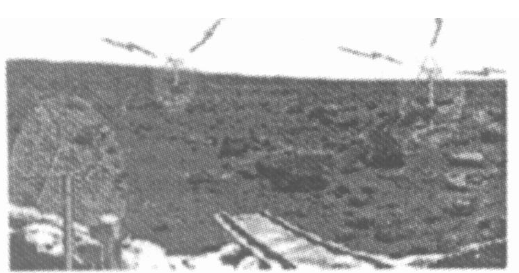
\includegraphics[width=0.65\textwidth]{../img/huoxing.png}
      %文件路径
      \caption*{火星上的伪卫星阵列}
      \label{fig:sb}    %(伏笔
    \end{figure}
\end{lstlisting}    
\end{framed}

效果如下:

\begin{figure}[htbp]
    \centering
    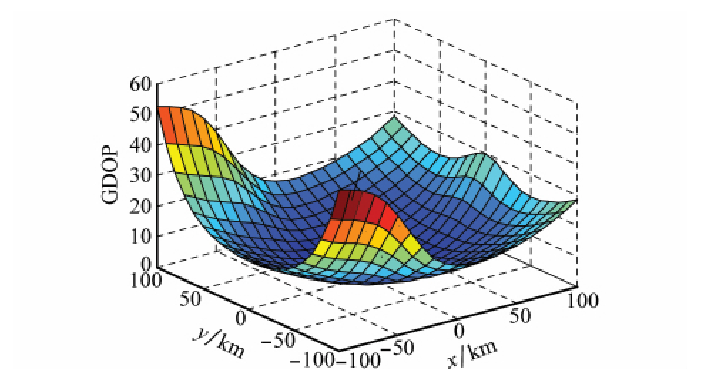
\includegraphics[width=0.65\textwidth]{../img/fz.png}
    \caption{某仿真图像}
    \label{fig:sb}
\end{figure}

注意一下代码里的{\textbackslash}label{\{fig:sb\}},后面引用的时候来个前后呼应。

我们还可以自定义环境,用法是

\begin{framed}
\begin{lstlisting}[language=]
    \newenvironment{新环境名称}[参数个数][参数默认值]
    {开始部分定义}{结束部分定义}
\end{lstlisting}
\end{framed}

有点像C/C++中的宏,新环境的开始部分和结束部分定义的内容在编译时被替换。如果要做一个“摘要”的新环境,可以这么设置并调用:

\begin{framed}
\begin{lstlisting}[language=]
    \newenvironment{Abstract}
    {
	\begin{center}\normalfont\bfseries Abstract\end{center}
	\begin{quote}\par
    }
    {\end{quote}}
    ......
    \begin{Abstract}
        This is an abstract Abstract.
    \end{Abstract}
\end{lstlisting}
\end{framed}

\newenvironment{Abstract}
{
    \begin{center}\normalfont\bfseries Abstract\end{center}
    \begin{quote}\par
}
{\end{quote}}

效果:(框是加的)

\begin{framed}
\begin{Abstract}
    This is an abstract Abstract.
\end{Abstract}
\end{framed}

再康康数院学长做的习题环境:

\begin{framed}
\begin{lstlisting}[language=]
    \definecolor{shadecolor}{RGB}{222, 227, 230}
    \newcounter{problemname}%计数器,用来标号
    \newenvironment{problem}
    {\begin{shaded}\stepcounter{problemname}\par\noindent
        \textbf{FRAME-\arabic{problemname}. }}
    {\end{shaded}\par}
    %shaded是framed包自带的底色环境
\end{lstlisting}
\end{framed}

\definecolor{shadecolor}{RGB}{222, 227, 230}
\newcounter{problemname}%计数器,用来标号
\newenvironment{problem}
    {
        \begin{shaded}\stepcounter{problemname}\par\noindent\textbf{FRAME-\arabic{problemname}. }
    }
    {\end{shaded}\par}

效果:

\begin{problem}
    已有3个学生的3门课成绩,分别用函数实现以下功能:

    1)计算每个学生的总成绩

    2)按照学生总成绩从高到低进行排序

    要求:

    1)在main函数中分别调用以上函数,按照学生三门课程总成绩从大到小输出学生的相关信息。

    2)函数自行定义。三个学生的信息按照如下直接赋值:

    1001,11,zhang,99.5,88.5,89.5

    1002,22,li,77.9,56.5,87.5

    1003,11,wang,92.5,99.0,60.5
\end{problem}

\section{代码}
当然对我来说,{\TeX}主要是用来记录CS学习的,所以不可避免地要插入很多代码。在{\TeX}中,使用lstlisting宏包来进行代码插入。这个宏包通过lstset来设置样式,支持100多种计算机语言的关键字高亮,还有各种背景色的样式设置等等。上面的代码中,我只简单设置了一下样式,边框则是通过framed宏包添加的。

来试试看自己调一个:

\lstset
{%
    language=C++, %语言种类
    frame=shadowbox, %边框预设
    xleftmargin=1.5em, %整体距左侧边线的距离为2em
    rulesepcolor=\color{lightgray}, %阴影颜色
    rulecolor=\color{black}, %框架颜色设置
    aboveskip=30pt, %与整个代码环境上面距离
    belowskip=10pt, %*下面
    breaklines=true, %自动换行
    basicstyle=\tt, %使用等宽字体,可调
    keywordstyle=\bfseries\color{green!40!black}, %设置关键字颜色为绿色,转变成bold加粗序列
    commentstyle=\itshape\color{purple!40!black}, %注释颜色设置为灰色
    identifierstyle=\color{blue}, %标识符设置为蓝色
	stringstyle=\color{orange}, %字符串设置为橙色
    showstringspaces=false, %去掉空格时产生的下划的空格标志, 设置为true则出现
    numbers=left, %在左侧显示行数
    numberstyle=\tiny\color{red}, %数字大小,颜色调整
    numberstyle=\it, %数字字体设为罗马斜体
    stepnumber=1 , %每行标号一次
    numbersep=10pt, %数字右端(若为左侧显示数字)水平距离代码5pt
    tabsize=4, %制表符长度
    framexleftmargin=0mm, %框架左边界延长
    framexrightmargin=-1mm, %框架右边界延长
    columns=fixed, %紧凑排列
}

\begin{framed}
\begin{lstlisting}[language=]
\lstset
{%
    language=C++, %语言种类
    frame=shadowbox, %边框预设
    xleftmargin=1.5em, %整体距左侧边线的距离为2em
    rulesepcolor=\color{lightgray}, %阴影颜色
    rulecolor=\color{black}, %框架颜色设置
    aboveskip=30pt, %与整个代码环境上面距离
    belowskip=10pt, %*下面
    breaklines=true, %自动换行
    basicstyle=\tt, %使用等宽字体,可调
    keywordstyle=\bfseries\color{green!40!black}, %设置关键字颜色为绿色,转变成bold加粗序列
    commentstyle=\itshape\color{purple!40!black}, %注释颜色设置为灰色
    identifierstyle=\color{blue}, %标识符设置为蓝色
    stringstyle=\color{orange}, %字符串设置为橙色
    showstringspaces=false, %去掉空格时产生的下划的空格标志, 设置为true则出现
    numbers=left, %在左侧显示行数
    numberstyle=\tiny\color{red}, %数字大小,颜色调整
    numberstyle=\it, %数字字体设为罗马斜体
    stepnumber=1 , %每行标号一次
    numbersep=10pt, %数字水平距离代码10pt
    tabsize=4, %制表符长度
    framexleftmargin=0mm, %框架左边界延长
    framexrightmargin=-1mm, %框架右边界延长
    columns=fixed, %紧凑排列
}

\begin{framed}
\begin{lstlisting}[language=C++]
    #include <stdio.h>

    int main(void)
    {
        int* nums;
        scanf("%d", nums);
    }
\ end{lstlisting}
\end{framed}
\end{lstlisting}
\end{framed}

输出:

\begin{framed}
\begin{lstlisting}[language=C++]
    #include <stdio.h>

    int main(void)
    {
        int* nums;
        scanf("%d", nums);
    }
\end{lstlisting}
\end{framed}

2023.4.1凌晨,调了3个小时。这下小丑了。

\section{公式}
公式是{\LaTeX}中的一种特殊环境,分为行内和行间公式两种。利用{\LaTeX},我们可以方便地对公式进行排版、对齐和交叉引用,唯一的不足是编辑起来实在是过于麻烦了,而且可能出现编译性的错误。好在Code给我们提供了一些脚本,也可以用前面提到的{\href{https://www.latexlive.com/}{公式生成器}}。

行内公式的样式与行间略有不同。输入{$\backslash$}lim{\_{}}{\{n{$\backslash$to}{$\backslash$}infty\}}和{$\backslash$}prod{\_{}}{\{n=1\}{\^{}}{\{{$\backslash$}infty\}}},效果如下:

\begin{framed}
行内公式:
    $\lim_{n\to\infty}$\qquad
    $\prod_{n=1}^{\infty}$

行间公式:
    $$\lim_{n\to\infty}{\qquad}\prod_{n=1}^{\infty}$$
\end{framed}

如果想让行内公式具有行间公式的样式,则加上{\textbackslash}limits或{\{{\textbackslash}displaystyle\}},如

\begin{framed}
\begin{lstlisting}[language=tex]
    \lim\limits_{n\to\infty}
    {\displaystyle\sum_{n=1}^{\infty}}
\end{lstlisting}
\end{framed}
效果:
    $\lim\limits_{n\to\infty}\qquad
    {\displaystyle\sum_{n=1}^{\infty}}$

关于括号的使用,直接使用 {(),[],\{\}},括号的高度不会随着括号中的内容高度而变化,如$(\frac{3}{\frac{114}{514}})^2$、$[\frac{1919^2}{810}]$,所以使用{\textbackslash}left{(\dots{\textbackslash}right)},效果:$\left(\frac{3}{\frac{114}{514}}\right)^2$。注意{\textbackslash}left(和{\textbackslash}right)必须成对出现,如果不想显示某一边则要把括号改成小数点,写成{\textbackslash}left[\dots{\textbackslash}right.。效果:$\left[\frac{1919^2}{810}\right.$

{\par}
行内公式调用如$ E=mc^2 $只需要{\$}E=mc{\^{}}2{\$}即可。

{\par}
行间公式调用有两种方法:

\begin{multicols*}{2}
\columnseprule 1pt  %中央分割线宽
\columnsep 40pt
\begin{enumerate}
    \item 使用{\textbackslash}[\dots{\textbackslash}]或者{\$\$\dots\$\$}这两种方法都只能输入单行公式,{\textbackslash}{\textbackslash}在其中失效。
    \item 使用环境,如:
        \begin{itemize}
            \item align
            \item alignat
            \item flalign
            \item equation
            \item gather
            \item multiline
        \end{itemize}
        使用环境公式的好处是可以自动编号并方便排版,打上label后也方便交叉引用。所有上面的环境都可以在环境名后面加*表示无序号。
\end{enumerate}
\end{multicols*}

先以align为例:

\begin{framed}
\begin{lstlisting}[language=]
\begin{align}
    &\ x~4+2x~3+11x~2+18x+18 \\
   =&\(x~2+2x+2)(x~2+9) \notag\\ 
   =&\(x~2+x+3)~2+(2x+3)~2
\end{align}
\end{lstlisting}
\end{framed}

环境中以{\$}为对称处标识符,整体中心对称{\textbackslash}{\textbackslash}表示换行,用{\textbackslash}notag或{\textbackslash}nonumber来隐藏任意一行公式的编号。效果:

\begin{align}
    &x^4+2x^3+11x^2+18x+18 \\
   =&(x^2+2x+2)(x^2+9) \notag\\ 
   =&(x^2+x+3)^2+(2x+3)^2
\end{align}

equation环境其实也只能插入一行公式,但是可以用spilt嵌套,好处是多行公式只显示一个编号。

\begin{framed}
\begin{lstlisting}[language=]
    \begin{equation}
        \label{eq1}
        \begin{split}
            &x^4+2x^3+11x^2+18x+18 \\
           =&(x^2+2x+2)(x^2+9) \\ 
           =&(x^2+x+3)^2+(2x+3)^2
        \end{split}
    \end{equation}
\end{lstlisting}
\end{framed}

效果:

\begin{equation}
    \label{eq1}
    \begin{split}
        &x^4+2x^3+11x^2+18x+18 \\
       =&(x^2+2x+2)(x^2+9) \\ 
       =&(x^2+x+3)^2+(2x+3)^2
    \end{split}
\end{equation}

除此之外,aligant和align环境没有什么区别;gather环境中不能出现对齐符号{\&},公式全部居中。case环境用于联立方程:

\begin{framed}
\begin{lstlisting}[language=]
    \begin{align*}
        \boxed{ %给公式加边框
        \begin{cases}
            2x + 3y = 7 \\
            3x + 5y = 8
        \end{cases}
        }
    \end{align*}
\end{lstlisting}
\end{framed}

效果:
\begin{align*}
    \boxed{
    \begin{cases}
        2x + 3y = 7 \\
        3x + 5y = 8
    \end{cases}
    }
\end{align*}

还有一种multiline环境,用的较少。

\begin{framed}
\begin{lstlisting}[language=]
    numberwithin{equation}{section} %编号带上section的序号
    \begin{multline}
        \text{字字字字字字} \\ %汉字必须这样括起来
        1-line \\
        2-line \\
        3-line \\
        4-line
    \end{multline}
\end{lstlisting}
\end{framed}

\begin{framed}
\numberwithin{equation}{section} %编号带上section的序号
\begin{multline}
    \text{字字字字字字} \\ %汉字必须这样括起来
    1-line \\
    2-line \\
    3-line \\
    4-line
\end{multline}
\end{framed}

最后是矩阵和行列式的输入:

\begin{framed}
\begin{lstlisting}[language=]
    \begin{center}
        $%注意要夹好
        \begin{pmatrix}
            a_{11} & a_{12} & \cdots & a_{1n} \\
            a_{21} & a_{22} &        & \vdots \\
            \vdots &        & \ddots & \vdots \\
            a_{n1} & \cdots & \cdots & a_{nn}
        \end{pmatrix}
        $
        $
        \begin{bmatrix}
            a_{11} & a_{12} \\
            a_{21} & a_{22} \\
        \end{bmatrix}
        $
        $\begin{vmatrix}
            a_{11} & a_{12} \\
            a_{21} & a_{22} \\
        \end{vmatrix}
        $
        $
        \begin{matrix}
            a_{11} & a_{12} \\
            a_{21} & a_{22} \\
        \end{matrix}
        $
        $
        \begin{Bmatrix}
            a_{11} & a_{12} \\
            a_{21} & a_{22} \\
        \end{Bmatrix}
        $
        $
        \begin{Vmatrix}
            a_{11} & a_{12} \\
            a_{21} & a_{22} \\
        \end{Vmatrix}
        $
        \end{center}
\end{lstlisting}
\end{framed}

效果:
\begin{center}
$%注意要夹好
\begin{pmatrix}
    a_{11} & a_{12} & \cdots & a_{1n} \\
    a_{21} & a_{22} &        & \vdots \\
    \vdots &        & \ddots & \vdots \\
    a_{n1} & \cdots & \cdots & a_{nn}
\end{pmatrix}
$
$
\begin{bmatrix}
    a_{11} & a_{12} \\
    a_{21} & a_{22} \\
\end{bmatrix}
$
$\begin{vmatrix}
    a_{11} & a_{12} \\
    a_{21} & a_{22} \\
\end{vmatrix}
$
$
\begin{matrix}
    a_{11} & a_{12} \\
    a_{21} & a_{22} \\
\end{matrix}
$
$
\begin{Bmatrix}
    a_{11} & a_{12} \\
    a_{21} & a_{22} \\
\end{Bmatrix}
$
$
\begin{Vmatrix}
    a_{11} & a_{12} \\
    a_{21} & a_{22} \\
\end{Vmatrix}
$
\end{center}

\section{表格}
在写文章的时候表格和公式一样重要。当然,表格最重要的用途还是记录实验数据,这个时候我们就可以打个三线表(需要booktabs宏包)先:

\begin{framed}
\begin{lstlisting}[language=]
    \begin{table*}
        \centering
        \begin{tabular}{llllll}%控制表格格式
            \toprule%一线
            睡觉 & 1$( km/s^2  )$ & & & & Sb \\
            \midrule%二线
            $\mathbb{C}$ & Test \\
            ? & & \\ %表格一定要在底线前换行
            \bottomrule%三线
        \end{tabular}
        \caption{睡觉工程学导论}
        \label{tbl:table1}
    \end{table*}    
\end{lstlisting}
\end{framed}

\begin{table*}[htb]
    效果:\\
    \centering
    \begin{tabular}{llllll}
        \toprule
        睡觉 & 1$( km/s^2  )$ & & & & Sb \\
        \midrule
        $\mathbb{C}$ & Test \\
        ? & & \\
        \bottomrule
    \end{tabular}
    \caption{睡觉工程学导论}
    \label{tbl:table1}
\end{table*}
    
如果是需要竖线的表,要合并单元格(需要multirow宏包),并使用创建框线的指令。

\begin{framed}
\begin{lstlisting}[language=]
    \multirow{NUMBER_OF_ROWS}{WIDTH}{CONTENT}
    %NUMBER_OF_ROWS代表该表格单元占据的行数,WIDTH代表表格的宽度,一般填 * 代表自动宽度,CONTENT则是表格单元里的内容。
    \multicolumn{NUMBER_OF_COLUMNS}{ALIGNMENT}{CONTENT}
    %NUMBER_OF_COLUMNS代表该表格单元占据的列数,ALIGNMENT代表表格内容的偏移(填l,c或者r),CONTENT则是表格单元里的内容。


    \begin{table}[htb]%浮动格式
        \centering
        \begin{tabular}{|c|c|c|c|c|c|c|c|}
        %在这些竖线中间,c表示中间对称,r、l以此类推
        \hline
        title & title2 & title3 & title4 & \multicolumn{4}{c|}{title5} \\%向右合并,共4列,内容居中
        \hline
        \multirow{5}{*}{1} & \multirow{5}{*}{column2} & \multirow{5}{*}{clo3} & \multirow{5}{*}{clo4}
        & f1 & f2 & f3 & f4 \\%向下合并,共5行,自动宽度
        \cline{5-8}
        & & & & 1 & 2 & 3 & 4 \\
        \cline{5-8}   
        & & & & 5 & 6& 7 & 8 \\
        \cline{5-8}
        & & & & 1 & 2 & 3 & 4 \\
        \cline{5-8}
        & & & & 5 & 6& 7 & 8 \\
        \hline
    \end{tabular}
    \caption{The title of the table}
    \label{}
    \end{table}
\end{lstlisting}
\end{framed}

\begin{table}[htb]
    \centering
    \begin{tabular}{|c|c|c|c|c|c|c|c|}
    \hline
    title & title2 & title3 & title4 & \multicolumn{4}{c|}{title5} \\
    \hline
    \multirow{5}{*}{1} & \multirow{5}{*}{column2} & \multirow{5}{*}{clo3} & \multirow{5}{*}{clo4} 
    & f1 & f2 & f3 & f4 \\
    \cline{5-8}
    & & & & 1 & 2 & 3 & 4 \\
    \cline{5-8}   
    & & & & 5 & 6& 7 & 8 \\
    \cline{5-8}
    & & & & 1 & 2 & 3 & 4 \\
    \cline{5-8}
    & & & & 5 & 6& 7 & 8 \\
    \hline
\end{tabular}
\caption{The title of the table}
\label{}
\end{table}
    
\section{树状图}
要画分叉树的话主要用Qtree或者TikZ-qtree宏包,后者的功能更强大,但是需要会TiKZ(TikZ是\TeX 中画图表的非常强大的宏包,Code的插件边栏中也有对应脚本),等后面用到的时候再做一篇吧。先介绍qtree。

这个用法非常简单,输入\textbackslash usepackage\{ qtree\} 调用该拓展包。通过\textbackslash Tree[ ]开始画树——“.”之后写标签,“\textbackslash qroof{}”画三角形,比如:

\begin{framed}
\begin{lstlisting}[language=]
    \centering
    \Tree [.IP
    .DP
    [.I'
        [.VP 
            [.V' 
             [.V drew ]
              [.DP 
                [.D' [.D a ] .NP ]
              ]
            ]
        ]
    ]
]
\end{lstlisting}
\end{framed}

注意:每个“] ”前必须得有空格,不然系统就会报错。比如“[.V drew ]”不能写成“[.V drew]”。如果节点名称比较长,需要多行时,可以使用大括号包含来表示,否则会被当作子节点处理。

效果如下:

\begin{framed}
\centering
\Tree [.IP
    .DP
    [.I'
        [.VP 
            [.V' 
             [.V drew ]
              [.DP 
                [.D' [.D a ] .NP ]
              ]
            ]
        ]
    ]
]
\end{framed}

qtree-tikz的用法大同小异,我们用它来尝试绘制一个二叉树。

\begin{framed}
\begin{lstlisting}[language=]
    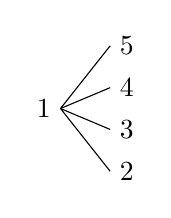
\begin{tikzpicture}[grow=right]%指定开口方向
        \centering
        \Tree
        [.1
        [.2 ] [.3 ] [.4 ] [.5 ] 
        ]
    \end{tikzpicture}
    % %加百分号把中间的换行符注释掉
    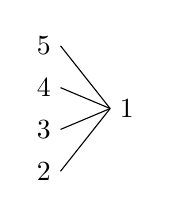
\begin{tikzpicture}[grow'=left]%grow'表示转置
        \Tree
        [.1
        [.2 ] [.3 ] [.4 ] [.5 ] 
        ]
    \end{tikzpicture}
    %
    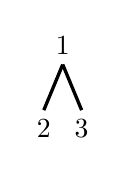
\begin{tikzpicture}
        \tikzset{edge from parent/.append style={very thick}}%设置线的样式
        \Tree
        [.1
        [.2 ] [.3 ]
        ]
    \end{tikzpicture}
    %
    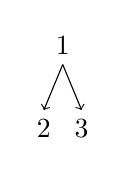
\begin{tikzpicture}[semithick,->]%加箭头
        \Tree
        [.1
        [.2 ] [.3 ]
        ]
    \end{tikzpicture}
    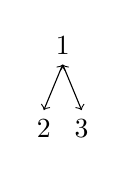
\begin{tikzpicture}[semithick,<->]%加箭头
        \Tree
        [.1
        [.2 ] [.3 ]
        ]
    \end{tikzpicture}
    %
    \begin{tikzpicture}[dashed]%虚线
        \Tree
        [.1
        [.2 ] [.3 [.4 5 6 ] ]
        ]
    \end{tikzpicture}
\end{lstlisting}
\end{framed}

效果:

\begin{framed}
\centering
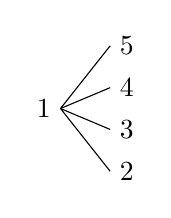
\begin{tikzpicture}[grow=right]%指定开口方向
    \Tree
    [.1
    [.2 ] [.3 ] [.4 ] [.5 ] 
    ]
\end{tikzpicture}
% %加百分号把中间的换行符注释掉
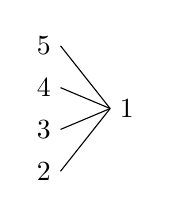
\begin{tikzpicture}[grow'=left]%grow'表示转置
    \Tree
    [.1
    [.2 ] [.3 ] [.4 ] [.5 ] 
    ]
\end{tikzpicture}
%
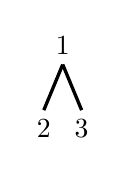
\begin{tikzpicture}
    \tikzset{edge from parent/.append style={very thick}}%设置线的样式
    \Tree
    [.1
    [.2 ] [.3 ]
    ]
\end{tikzpicture}
%
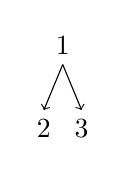
\begin{tikzpicture}[semithick,->]%加箭头
    \Tree
    [.1
    [.2 ] [.3 ]
    ]
\end{tikzpicture}
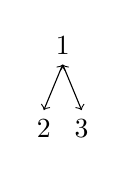
\begin{tikzpicture}[semithick,<->]%加箭头
    \Tree
    [.1
    [.2 ] [.3 ]
    ]
\end{tikzpicture}
%
\begin{tikzpicture}[dashed]%虚线
    \Tree
    [.1
    [.2 ] [.3 [.4 5 6 ] ]
    ]
\end{tikzpicture}
\end{framed}

\section{页面设置}
可以如此设置页边距和行距:

\begin{framed}
\begin{lstlisting}[language=]
    \linespread{0.5}    %设置{n}倍行距
    \geometry{left=1.0cm, right=1.0cm, top=0.5cm, bottom=0.5cm}%设定页边距
\end{lstlisting}
\end{framed}

以及前面提到的多栏环境:

\begin{framed}
    \begin{lstlisting}
        \begin{multicols}{2}%2是栏数
        \columnseprule 1pt  %中央分割线宽
        \columnsep 35pt     %控制两栏之间间隔
        无序列表
        \begin{itemize}
            \item 我是SB
            \item SB is me.
            \item Sb is xjtu.
        \end{itemize}
        有序列表
        \begin{enumerate}
            \item 主E20楼
            \item 一跃解千愁{\label{sb}}
        \end{enumerate}
        \end{multicols}
    \end{lstlisting}
    \end{framed}

现在会套模板已经够用了,最多就是加个多栏环境。
    
至于像学术期刊那样那么漂亮的排版,后面还会补的(吧?)。

\section{引用}
最后是\LaTeX 最为强大的功能之一:交叉引用。使用到了hyperref宏包。

在每个环境的end之前,通过\textbackslash labal\{ name\} 指令将环境的内部名称指定为name,然后我们们可以直接通过\textbackslash ref指令进行文内引用。比如上面提到的伏笔:\ref{fig:sb}。

这个1是自动生成的,感觉有点大,我们自定义一个\textbackslash upref命令让数字显示在右上角\upref{fig:sb} 。

\begin{lstlisting}
    \newcommand{\upref}[1]{\textsuperscript{\ref{#1}}}
\end{lstlisting}

使用hyperref宏包还可以链接
\href{https://space.bilibili.com/16725323}{外部网站}和
\href{run:/sample.bib}{本地文件}
,格式如下:

\begin{lstlisting}
    使用hyperref宏包还可以链接
    \href{https://space.bilibili.com/16725323}{外部网站}和
    \href{run:/sample.bib}{本地文件}
\end{lstlisting}

关于参考资料的外部引用,则是使用的\textbackslash cite指令,同样自定义一个\textbackslash upcite指令。当然我们要先创建参考资料环境:

\begin{lstlisting}
    \begin{thebibliography}{99}
        \bibitem{a}作者. \emph{文献}[M]. 地点:出版社,年份.
        \bibitem{b}作者. \emph{文献}[M]. 地点:出版社,年份.
    \end{thebibliography}
\end{lstlisting}

\begin{lstlisting}
    \newcommand{\upcite}[1]{\textsuperscript{\cite{#1}}}
\end{lstlisting}

然后引用\upcite{ref1} 。注意这种方法需要两次以上编译。

另外一种方法是以bibtex来管理文献,这种方法很适合批量管理文献。为此,要创建一个\href{run:./sample.bib}{sample.bib} 文件,里面像json一样写入了文献的信息。例如:

\begin{framed}
\begin{lstlisting}
    @article{12,%12是这篇文献的label
    title            = {基于无迹卡尔曼滤波的室内定位系统},
    author           = {王袁雪;张前波;周媛媛;刘英明;李冰},
    authoraddress    = {河北师范大学中燃工学院},
    journal          = {物联网技术},
    year             = {2022},
    volume           = {12},
    number           = {07},
    pages            = {18-19},
    keywords         = {室内定位;超宽带;无迹卡尔曼滤波;非视距;chan算法;二维地图},
    isbn/issn        = {2095-1302},
    notes            = {61-1483/tp},
    doi              = {10.16667/j.issn.2095-1302.2022.07.005},
    databaseprovider = {cnki}
    }
\end{lstlisting}
\end{framed}

然后在文章末尾指定bib数据库文件和样式:

\begin{lstlisting}
    \bibliographystyle{IEEEtran}
    \bibliography{sample.bib}
\end{lstlisting}

开始愉快地引用吧\upcite{12} ,至于排号和文献的先后顺序\upcite{001} ,bib会帮你排好的\upcite{002} 。不过要同样注意:bibtex需要xe→bib→xe→xe这样编译数次。以及这篇文档因为用了两种方式,所以出现了两个“参考文献”。

\section{常用模板}\label{sec:preset}
最后终于来到了模板介绍时间。现在做了四个互相补充的模板:
\begin{itemize}
    \item 平时作业
        \begin{itemize}
            \item 用于平时选修课的作业
            \item 使用bib管理参考文献,排版已经排好
        \end{itemize}
    \item 数模论文
        \begin{itemize}
            \item 大佬分享的建模论文模板
            \item 在文件夹中附上了mcode宏包,支持MATLAB代码
            \item 自定义了论文写作时要用的多种环境
        \end{itemize}
    \item 数学习题
        \begin{itemize}
            \item 提供了带有底色的问题-解答-评注环境
            \item 可以按照自己意愿修改配色方案
        \end{itemize}
    \item 代码
        \begin{itemize}
            \item 调好了代码样式和配色
            \item 主要支持C/C++语言种类
            \item 很适合学习CS时拿来记笔记
        \end{itemize}
\end{itemize}

终于结束了,如果你是除了Shiyuu以外的阅读者,必须感谢你读到这里。这只是我个人到目前为之有需求的地方,不免有遗漏和偏颇,排版和屁话让这篇文档又臭又长且可能有点自说自话,但还是希望这篇自用的文档能有所帮助。

%%%%%%%%%%%%%%%%%%%%%%%%%%%%%%%%%%%%%%%%%%%%%%%%%%%%%%%%%%%%%%%%%%%%%%%%%%%
\begin{thebibliography}{99}
    \bibitem{ref1} https://zhuanlan.zhihu.com/p/379321421.
\end{thebibliography}

\bibliographystyle{IEEEtran}
\bibliography{sample.bib}

\end{document}